\section{Mass Budget Breakdown}
\label{DDMBB}
The table \ref{tab:MB} on page \pageref{tab:MB} indicates mass budget breakdown for emitter and receiver satellites. The table is mainly divided into two parts. The first part gives each subsystem mass of emitter and receiver satellites in both kilograms and percentage of total dry mass. Meanwhile, the second part includes the mass of propellants and then also gives the total mass when the satellites are in their orbit. The derivation of all numbers in the table can be found in each corresponding chapter of the subsystem.

\begin{table}[h!]
\centering
\begin{tabular}{|l|c|c|c|c|}
\hline
 & \multicolumn{2}{|c|}{Emitter} & \multicolumn{2}{|c|}{Receiver} \\\hline
 Subsystem        & $M [kg]$ & \%$M_{dry}$ & $M [kg]$ & \%$M_{dry}$ \\\hline\hline
 Communication    & 10.66    & 21          & 3        & 22.2 \\\hline
 Navigation       & 0.25     & 0.5         & 0.25     & 1.85 \\\hline
 OEP              & 15       & 29.8        & -        & - \\\hline
 ORP              & 0.22     & 0.4         & 0.22     & 1.63 \\\hline
 EPS              & 5.8      & 11.5        & 3.6      & 26.6 \\\hline
 ADCS             & 2        & 4           & 2        & 14.8 \\\hline
 Thermal          & 1.48     & 3           & 0.3      & 2.22 \\\hline
 Structure        & 12.35    & 24.5        & 2.45     & 18.12 \\\hline
 Propulsion(tank) & 1        & 2           & 0.75     & 5.55 \\\hline
 Thruster         & 0.65     & 1.3         & 0.15     & 1.11 \\\hline
 Shielding        & 1        & 2           & 0.8      & 5.92 \\\hline\hline
 $M_{dry}$        & 50.41    & 100         & 13.52    & 100 \\\hline
 $M_{propellant}$ & 4        & -           & 1.5      & - \\\hline
 $M_{Loaded}$     & 54.41    & -           & 15.02    & - \\\hline
 $M_{Orbit}$      & 53.1     & -           & 14.92    & - \\\hline
\end{tabular}
\caption{Mass Budget Breakdown of the emitter and a representative receiver satellite.}
\label{tab:MB}
\end{table}

As discussed in section \ref{frRecDV}, the receivers would need different propellant masses. Table \ref{tab:MB} on page \pageref{tab:MB} displays the maximum receiver loaded mass, and mass in orbit is the same for all.

%%%%%%%%%%%%%%%%%%%%%%%%%%%%%%%%%%%%%%%%%%%%%%%%%%%%%%%%%%%%%%%%%%%%%%%%%%%%%%%%%%%%%%%%%%%%%
\section{Cost Budget Breakdown}
\label{DDCB}
Figure \ref{fig:lifecycle} on page \pageref{fig:lifecycle} shows the typical life-cycle for a space mission. The \ac{RDTE} stage includes the planning, development and testing of all prototypes and qualification units, but does not include the technology development for different subsystems. In the case of the laser swarm this is largely dependent on the single emitter and one receiver unit. This stage is also mostly consistent of non-recurring costs. The production stage consists of actual manufacture of the physical satellites. The cost estimation in this stage is based on the \ac{TFU}. This is done because it is assumed that the first unit (in the case of the Laser Swarm, that would be the emitter and one receiver) would be the most expensive to produce. The rest of the swarm constellation satellite costs are calculated by taking a theoretical learning curve \cite{larson}. 

\begin{figure}[ht!]
\centering
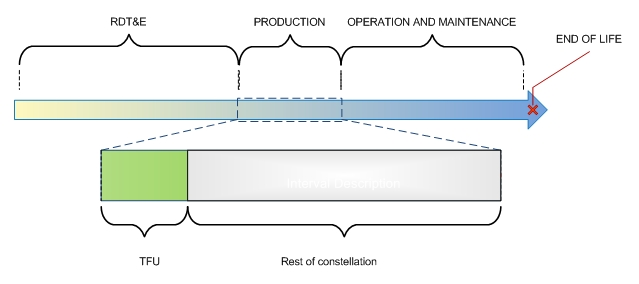
\includegraphics[scale = 0.8]{chapters/img/lifetime.jpg}
\caption{Satellite Life-Cycle}
\label{fig:lifecycle}
\end{figure}

Table \ref{tab:CB} on page \pageref{tab:CB} gives the cost breakdown of both theoretical first unit cost for emitter and receiver satellites and also the swarm of 9 satellites including all the wraps.

\begin{table}[ht!]
\centering
\begin{tabular}{l|c|c|c|c|c|c|}
\cline{2-7}
  & \multicolumn{4}{|c|}{Unit Cost} & \multicolumn{2}{|c|}{\multirow{2}{*}{Swarm (9 satellites)}} \\\cline{2-5}
  
  & \multicolumn{2}{|c|}{Emitter satellite} & \multicolumn{2}{|c|}{Receiver satellite} & \multicolumn{2}{|c|}{ } \\\hline
  
 \multicolumn{1}{|c|}{Subsystem} & Cost [k\$] & \%Subtotal & Cost [k\$] & \%Subtotal & Cost [k\$] & \%Subtotal \\\hline
                                     %  cost [k$] %Total 
 \multicolumn{1}{|l|}{\textbf{Payload}}       & 8215.96 & 41.5 & 4048.74 & 46.58 & 8660 & 25.3 \\\hline
 \multicolumn{7}{|l|}{\textbf{Bus Total}}     \\\hline
 \multicolumn{1}{|l|}{Structure}     & 1920.38 & 9.7 & 843.2 & 9.7 & 3322.33 & 9.7 \\\hline
 \multicolumn{1}{|l|}{Thermal}       & 217.776 & 1.1 & 95.62 & 1.1 & 376.76 & 1.1 \\\hline
 \multicolumn{1}{|l|}{EPS}           & 541 & 2.7 & 266 & 3.06 & 1193.694 & 3.49 \\\hline
 \multicolumn{1}{|l|}{Navigation}    & 25   & 0.13 & 25 & 0.29 & 191.235 & 0.558 \\\hline
 \multicolumn{1}{|l|}{Communication} & 2940 & 14.9 & 612.5 & 7.05 & 7141.14 & 20.85 \\\hline
 \multicolumn{1}{|l|}{\acs{ADCS}}    & 199.093 & 1 & 175.914 & 2.02 & 1405.687 & 4.1 \\\hline
 \multicolumn{1}{|l|}{Tank}          & 0.713 & 0.0036 & 0.428 & 0.0049 & 3.649 & 0.011 \\\hline
 \multicolumn{1}{|l|}{Thruster}      & 570.64  & 2.88 & 356.65  & 4.1 & 3016.9 & 8.8 \\\hline
 \multicolumn{7}{|l|}{\textbf{Wraps}}     \\\hline
 \multicolumn{1}{|l|}{\acs{IAT}}     & 1445.24 & 7.3 & 634.58 & 7.3 & 2500.34 & 7.3 \\\hline
 \multicolumn{1}{|l|}{Program Level} & 2395.53 & 12.1 & 1051.84 & 12.1 & 4144.36 & 12.1 \\\hline
 \multicolumn{1}{|l|}{\acs{GSE}}     & 692.92 & 3.5 & 304.25 & 3.5 & 1198.78 & 3.5 \\\hline
 \multicolumn{1}{|l|}{\acs{LOOS}}    & 633.53 & 3.2 & 278.17 & 3.2 & 1096.03 & 3.2 \\\hline
 \multicolumn{1}{|l|}{Subtotal}      & 19797.79 & 100 & 8692.92 & 100 & 34250.88 & 100 \\\hline
 \multicolumn{1}{|l|}{Launch}        & - & - & - & - & 18534.25 & - \\\hline\hline\hline
 \multicolumn{1}{|l|}{\textbf{Total}}         & - & - & - & - & 52785.13 & - \\\hline
 \multicolumn{1}{|l|}{\textbf{Total (FY00)}}  & - & - & - & - & 43089.90 & - \\\hline
 
\end{tabular}
\caption{Cost Budget Breakdown.}
\label{tab:CB}
\end{table}